\documentclass{beamer}

\usetheme{Madrid} % Singapore, Madrid, Ilmenau, CambridgeUS
\setbeamertemplate{navigation symbols}{}

% --- Colores personalizados ---
\definecolor{unahurverde}{HTML}{005C5C}
\definecolor{unahurgris}{HTML}{EAEAEA}
\setbeamercolor{structure}{fg=unahurverde}
\setbeamercolor{frametitle}{bg=unahurverde, fg=white}
\setbeamercolor{title}{fg=unahurverde}
\setbeamercolor{block title}{bg=unahurverde, fg=white}
\setbeamercolor{block body}{bg=unahurgris, fg=black}

% --- Logo en esquina superior derecha ---
\addtobeamertemplate{frametitle}{}{%
	\begin{textblock*}{3cm}(11.88cm,0.12cm)
		
\includegraphics[height=0.7cm]{logo_unahur.png}
	\end{textblock*}
}

\setbeamertemplate{caption}[numbered]


\usepackage[utf8]{inputenc}
\usepackage[spanish]{babel}
\usepackage{graphicx}
\usepackage{ragged2e}
\usepackage[table]{xcolor}
\usepackage{listings}
\usepackage{caption}
%\usepackage{enumitem}
\usepackage[absolute,overlay]{textpos} % Necesario para el logo

\usefonttheme[onlymath]{serif}

\definecolor{codegray}{rgb}{0.5,0.5,0.5}
\definecolor{backcolor}{rgb}{0.95,0.95,0.95}
\definecolor{verdecelda}{HTML}{B7CBA6}
\definecolor{rojocelda}{HTML}{FF9999}
\definecolor{lightgray}{gray}{0.6}

\definecolor{codebg}{rgb}{0.95,0.97,0.98}       % fondo celeste muy suave
\definecolor{codecomment}{rgb}{0.42,0.55,0.34}  % verde oliva suave y cursiva
\definecolor{codekeyword}{rgb}{0.0,0.45,0.73}    % azul turquesa
\definecolor{codestring}{rgb}{0.78,0.36,0.14}   % naranja marrón claro
\definecolor{codenumber}{rgb}{0.5,0.5,0.5}      % gris numeración
\definecolor{coderule}{rgb}{0.7,0.8,0.9}        % borde celeste suave

\lstdefinestyle{mystyle}{
	backgroundcolor=\color{codebg},
	commentstyle=\color{codecomment},
	keywordstyle=\color{codekeyword}\bfseries,
	stringstyle=\color{codestring},
	numberstyle=\tiny\color{codenumber},
	basicstyle=\ttfamily\footnotesize,
	breaklines=true,
	captionpos=b,
	keepspaces=true,
	numbersep=7pt,
	showspaces=false,
	showstringspaces=false,
	showtabs=false,
	tabsize=2,
	inputencoding=utf8,
	extendedchars=true,
	frame=single,
	rulecolor=\color{coderule},
	numbers=none,
	xleftmargin=10pt,
	literate={π}{{$\pi$}}1 {θ}{{$\theta$}}1 {μ}{{$\mu$}}1 {β}{{$\beta$}}1 {η}{{$\eta$}}1 {δ}{{$\delta$}}1 {Δ}{{$\Delta$}}1
	{á}{{\'a}}1 {é}{{\'e}}1 {í}{{\'i}}1 {ó}{{\'o}}1 {ú}{{\'u}}1
	{Á}{{\'A}}1 {É}{{\'E}}1 {Í}{{\'I}}1 {Ó}{{\'O}}1 {Ú}{{\'U}}1
	{ñ}{{\~n}}1 {Ñ}{{\~N}}1 {ζ}{{$\zeta$}}1
}

\lstset{style=mystyle}

\lstset{
	language=Python,
	emph={self, _aplicar_gamma, _escalar_255, _generar_vector_ruido, _aplicar_ruido_sal_y_pimienta, _aplicar_ruido, _aplicar_ecualizacion_histograma, _aplicar_umbralizacion, _aplicar_negativo}, emphstyle=\color{purple}\bfseries,
}

\title{Trabajo Práctico 1 Procesamiento de Imágenes y Visión por Computadora}
\author{Matías Cisnero}
\date{11 de agosto de 2025}

\begin{document}
	
	% Portada
\begin{frame}
	\centering
	
\includegraphics[width=0.25\textwidth]{UNAHUR.png}
	\vfill
	{\huge \textbf{Trabajo Práctico 1}}\\[0.2cm]
	{\Large Procesamiento de Imágenes y Visión por Computadora}\\
	\vfill
	{\large Matías Cisnero}\\
	{\small 11 de agosto de 2025}
\end{frame}
	
\section{Ejercicio 1}
	
\begin{frame}
	\begin{center}
		\textcolor{unahurverde}{\textbf{Consigna 1:}}
	\end{center}
	\justifying
	
	Implementar la función de potencia $\gamma, 0 < \gamma < 2$ y $\gamma \neq 1$.
\end{frame}

\begin{frame}[fragile]{Transformación Gamma $\gamma$}
	\justifying

	\begin{block}{Definición}
		\[
		T(r) = c . r^\gamma, \quad 0 < \gamma < 2, \ \gamma \neq 1
		\]
	\end{block}
	
	Donde $c$ es una constante apropiada, de tal forma que $T(255) = 255$.
	
	\begin{block}{Constante $c$}
		\[
		c = 255^{1-\gamma}
		\]
	\end{block}
	
	Y $r$ los niveles de gris de una imagen $f$.
\end{frame}

\begin{frame}[fragile]{Código}
	\justifying
	
	\begin{lstlisting}[language=Python]
def _aplicar_gamma(self, imagen, gamma):
	# Convierto en un array de (m, n, 3)
	imagen_np = np.array(imagen)
			
	c = (255)**(1-gamma)
	resultado_np = c*(imagen_np**gamma)
			
	self.imagen_procesada = Image.fromarray(resultado_np.astype('uint8'))
	\end{lstlisting}
	
 \vfill
	\footnotesize \textcolor{lightgray}{(*) Se puede operar directamente con la imagen gracias al Broadcasting de Numpy (ver \cite{numpy-broadcasting}).}
\end{frame}

\begin{frame}[fragile]{Resultados}
	\justifying
	Al aplicar \textcolor{unahurverde}{\textbf{la transformación gamma}} con $\gamma = 1.5$ sobre la imagen de la Figura~\ref{fig:lenaoriginal1}, 
	se obtuvo la versión modificada que aparece en la Figura~\ref{fig:lenaej1}.
	\vspace{0.5cm}
	
	\centering
	\begin{minipage}{0.45\linewidth}
		\centering
		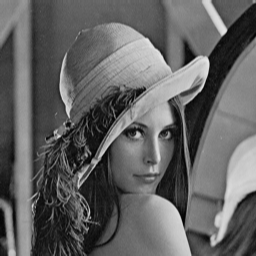
\includegraphics[width=\linewidth]{../results/lena_original}
		\captionof{figure}{Imagen original}
		\label{fig:lenaoriginal1}
	\end{minipage}\hfill
	\begin{minipage}{0.45\linewidth}
		\centering
		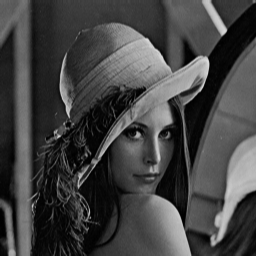
\includegraphics[width=\linewidth]{../results/lena_ej1}
		\captionof{figure}{Imagen modificada}
		\label{fig:lenaej1}
	\end{minipage}
\end{frame}

\section{Ejercicio 2}

\begin{frame}
	\begin{center}
		\textcolor{unahurverde}{\textbf{Consigna 2:}}
	\end{center}
	\justifying
	
	Implementar una función que devuelva el negativo de una imagen.
\end{frame}

\begin{frame}[fragile]{Negativo}
	\justifying
	
	\begin{block}{Definición}
		\[
		T(r) = 255 - r
		\]
	\end{block}
\end{frame}

\begin{frame}[fragile]{Código}
	\justifying
	
	\begin{lstlisting}[language=Python]
def _aplicar_negativo(self):
	# Convierto en un array de (m, n, 3)
	imagen_np = np.array(self.imagen_procesada)
	
	resultado_np = 255 - imagen_np
	self.imagen_procesada = Image.fromarray(resultado_np.astype('uint8'))
	\end{lstlisting}
	
	\vfill
	\footnotesize \textcolor{lightgray}{(*) Nuevamente se puede operar directamente gracias al Broadcasting de Numpy (ver \cite{numpy-broadcasting}).}
\end{frame}

\begin{frame}[fragile]{Resultados}
	\justifying
    Al aplicar \textcolor{unahurverde}{\textbf{la transformación de negativo}} sobre la imagen de la Figura~\ref{fig:lenaoriginal2}, 
    se obtuvo el resultado que se observa en la Figura~\ref{fig:lenaej2}.
	\vspace{0.5cm}
	
	\centering
	\begin{minipage}{0.45\linewidth}
		\centering
		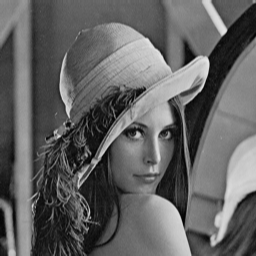
\includegraphics[width=\linewidth]{../results/lena_original}
		\captionof{figure}{Imagen original}
		\label{fig:lenaoriginal2}
	\end{minipage}\hfill
	\begin{minipage}{0.45\linewidth}
		\centering
		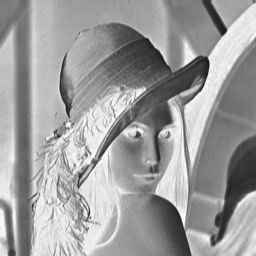
\includegraphics[width=\linewidth]{../results/lena_ej2}
		\captionof{figure}{Imagen en negativo}
		\label{fig:lenaej2}
	\end{minipage}
\end{frame}

\section{Ejercicio 3}

\begin{frame}
	\begin{center}
		\textcolor{unahurverde}{\textbf{Consigna 3:}}
	\end{center}
	\justifying
	
	Implementar una función que devuelva el histograma de niveles de gris de una imagen.
\end{frame}

\begin{frame}[fragile]{Histograma}
	\justifying
	
	\begin{block}{Definición}
		\[
		h_i = \frac{n_i}{N.M}, i=0,...,255
		\]
	\end{block}
	
	Donde
	
	\begin{itemize}
		\item $n_i:$ cantidad de ocurrencias del nivel de gris i dentro de la imagen.
		\item $NM$ cantidad total de píxeles de la imagen, M filas y N columnas.
	\end{itemize}
	
\end{frame}

\begin{frame}[fragile]{Resultados}
	\justifying
    Al graficar \textcolor{unahurverde}{\textbf{el histograma de niveles de gris}} de la imagen de la Figura~\ref{fig:lenaoriginal3}, 
    se obtuvo la representación que se muestra en la Figura~\ref{fig:lenaej3}.
	\vspace{0.5cm}
	
	\centering
	\begin{minipage}{0.45\linewidth}
		\centering
		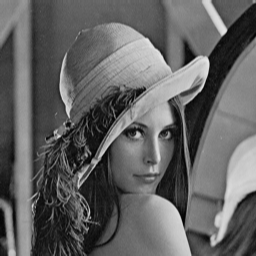
\includegraphics[width=\linewidth]{../results/lena_original}
		\captionof{figure}{Imagen original}
		\label{fig:lenaoriginal3}
	\end{minipage}\hfill
	\begin{minipage}{0.45\linewidth}
		\centering
		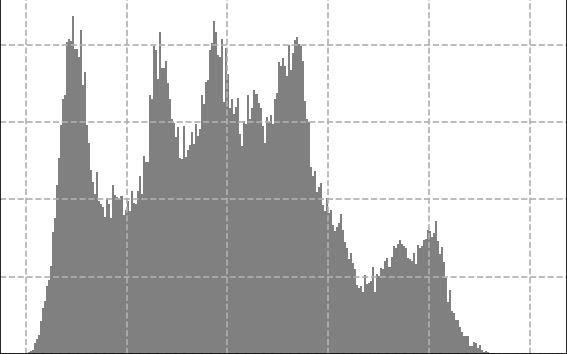
\includegraphics[width=\linewidth]{../results/lena_hist_gris}
		\captionof{figure}{Histograma de la imagen}
		\label{fig:lenaej3}
	\end{minipage}
\end{frame}

\section{Ejercicio 4}

\begin{frame}
	\begin{center}
		\textcolor{unahurverde}{\textbf{Consigna 4:}}
	\end{center}
	\justifying
	
	Implementar una función que aplique un umbral a una imagen, devolviendo una imagen binaria. El umbral debe ser un parámetro de entrada.
\end{frame}

\begin{frame}[fragile]{Umbralización}
	\justifying
	
	\begin{block}{Definición}
		Dado un umbral $u \in [0,...,255]$
		\[
		T(r) =
		\begin{cases}
			255, & \text{si } r \geq u \\
			0, & \text{si } r < u
		\end{cases}
		\]
	\end{block}
\end{frame}

\begin{frame}[fragile]{Código}
	\justifying
	
	\begin{lstlisting}[language=Python]
def _aplicar_umbralizacion(self, imagen, umbral):
	# Convierto en un array de (m, n, 3)
	imagen_np = np.array(imagen)
	
	resultado_np = np.where(imagen_np >= umbral, 255, 0)
	
	self.imagen_procesada = Image.fromarray(resultado_np.astype('uint8'))
	\end{lstlisting}
	
	\vfill
	\footnotesize \textcolor{lightgray}{(*) np.where es una forma vectorizada de hacer un if-else para los píxeles de la imagen (ver \cite{numpy.where}).}\\
	\footnotesize \textcolor{lightgray}{(*) El umbral se asigna mediante un Scale (slider) de tkinter.}
\end{frame}

\begin{frame}[fragile]{Resultados}
	\justifying
    Al aplicar la técnica de \textcolor{unahurverde}{\textbf{umbralización}} sobre la imagen de la Figura~\ref{fig:lenaoriginal4}, 
    con un valor de umbral de $u=128$, se obtuvo la imagen binaria que se muestra en la Figura~\ref{fig:lenaej4}.
	\vspace{0.5cm}
	
	\centering
	\begin{minipage}{0.45\linewidth}
		\centering
		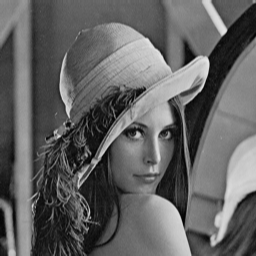
\includegraphics[width=\linewidth]{../results/lena_original}
		\captionof{figure}{Imagen original}
		\label{fig:lenaoriginal4}
	\end{minipage}\hfill
	\begin{minipage}{0.45\linewidth}
		\centering
		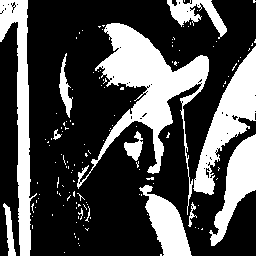
\includegraphics[width=\linewidth]{../results/lena_ej4}
		\captionof{figure}{Imagen binaria}
		\label{fig:lenaej4}
	\end{minipage}
\end{frame}

\section{Ejercicio 5}

\begin{frame}
	\begin{center}
		\textcolor{unahurverde}{\textbf{Consigna 5:}}
	\end{center}
	\justifying
	
	Implementar una función que realice la ecualización del histograma para mejorar la imagen.
\end{frame}

\begin{frame}[fragile]{Ecualización del histograma}
	\justifying
	
	\begin{block}{Definición}
		\[
		s_k = T(r_k) = \sum_{i=0}^{k} \frac{n_i}{n}
		\]
	\end{block}
	
	donde:
	
	\begin{itemize}
		\item $r_k$ es el k-ésimo nivel de gris dentro del intervalo [0, 255].
		\item $n_i$, $i=0,...,255$ es el número de pixels de la imagen con nivel de gris $r_i$, $i=0,...,255$.
		\item $n$ es el número total de pixels de la imagen.
		\item $\frac{n_i}{n}$, $i=0,...,255$ es la frecuencia relativa del i-ésimo nivel de gris.
	\end{itemize}
	
	Actualmente $s_{min} \leq s_k \leq 1$ y queremos que $s_k \in [0, 255]$, para eso aplicamos la siguiente transformación para discretizar los valores:
	
	\[
	\hat{s_k} = 255 * \lceil \frac{s_k - s_{min}}{1 - s_{min}} \rceil
	\]
\end{frame}

\begin{frame}[fragile]{Código}
	\justifying
	
	\begin{lstlisting}[language=Python]
def _aplicar_ecualizacion_histograma(self):
	imagen_np_gris = np.array(self.imagen_procesada.convert('L')) # Array de la forma (m. n).
	datos_gris = imagen_np_gris.flatten()
	
	n_r = np.bincount(datos_gris, minlength=256) # Freq abs(ni)
	NM = datos_gris.size # Pixels totales(n)
	h_r = n_r / NM # Freq relativa(ni/n)
	
	sk = np.zeros(256) # Hacemos la suma acumulada
	for k in range(len(sk)):
		sk[k] = np.sum(h_r[0:k+1])
	
	sk_sombrero = self._escalar_255(sk) # Discretizamos
	resultado_np = sk_sombrero[imagen_np_gris]
	
	self.imagen_procesada = Image.fromarray(resultado_np.astype('uint8')).convert('RGB')
	\end{lstlisting}
\end{frame}

\begin{frame}[fragile]{Código +}
	\justifying
	Una forma más optimizada de hacerlo aprovechando los métodos de Numpy.
	
	\begin{lstlisting}[language=Python]
def _aplicar_ecualizacion_histograma(self):
	imagen_np_gris = np.array(self.imagen_procesada.convert('L'))
	datos_gris = imagen_np_gris.flatten()
	
	n_r = np.bincount(datos_gris, minlength=256) # Freq abs
	h_r = n_r / np.sum(n_r) # Freq relativa
	
	sk = np.cumsum(h_r)
	sk_sombrero = self._escalar_255(sk) # Discretizamos
	
	resultado_np = sk_sombrero[imagen_np_gris]
	self.imagen_procesada = Image.fromarray(resultado_np.astype('uint8')).convert('RGB')
	\end{lstlisting}
	
	\vfill
	\footnotesize \textcolor{lightgray}{(*) np.cumsum hace la suma acumulada desde el principio hasta la posición del valor (ver \cite{numpy.cumsum}). np.bincount cuenta la cantidad de veces que aparece cada valor con indice igual a nivel de pixel y valor igual a frecuencia (ver \cite{numpy.bincount}).}
\end{frame}

\begin{frame}[fragile]{Resultados histogramas}
	\justifying
	Al aplicar \textcolor{unahurverde}{\textbf{la ecualización del histograma}} sobre el de la Figura~\ref{fig:hist_original}, 
	se obtuvo la versión ecualizada que se muestra en la Figura~\ref{fig:hist_ecualizado}.
	\vspace{0.5cm}
	
	\centering
	\begin{minipage}{0.45\linewidth}
		\centering
		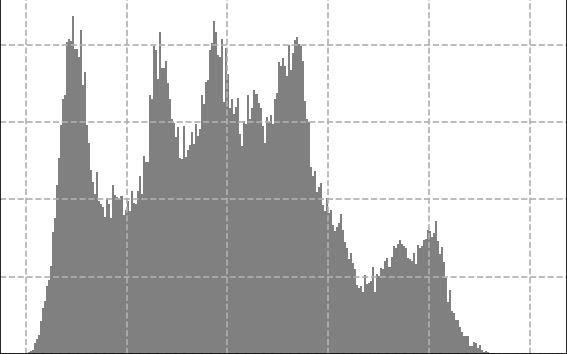
\includegraphics[width=\linewidth]{../results/lena_hist_gris}
		\captionof{figure}{Histograma original}
		\label{fig:hist_original}
	\end{minipage}\hfill
	\begin{minipage}{0.45\linewidth}
		\centering
		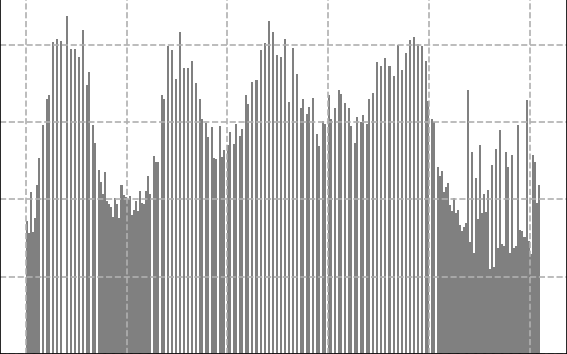
\includegraphics[width=\linewidth]{../results/lena_hist_gris_ecualizado}
		\captionof{figure}{Histograma ecualizado}
		\label{fig:hist_ecualizado}
	\end{minipage}
\end{frame}

\begin{frame}[fragile]{Resultados imagen}
	\justifying
	Al aplicar \textcolor{unahurverde}{\textbf{la ecualización}} sobre la imagen de la Figura~\ref{fig:lenaoriginal5}, 
	se obtuvo la versión mejorada que aparece en la Figura~\ref{fig:lenaej5}.
	\vspace{0.5cm}
	
	\centering
	\begin{minipage}{0.45\linewidth}
		\centering
		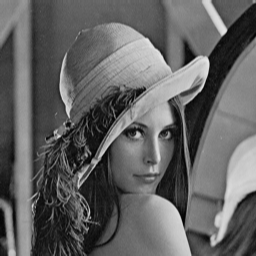
\includegraphics[width=\linewidth]{../results/lena_original}
		\captionof{figure}{Imagen original}
		\label{fig:lenaoriginal5}
	\end{minipage}\hfill
	\begin{minipage}{0.45\linewidth}
		\centering
		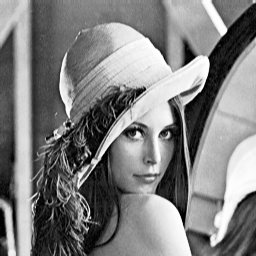
\includegraphics[width=\linewidth]{../results/lena_ej5}
		\captionof{figure}{Imagen ecualizada}
		\label{fig:lenaej5}
	\end{minipage}
\end{frame}

\section{Ejercicio 6}

\begin{frame}
	\begin{center}
		\textcolor{unahurverde}{\textbf{Consigna 6:}}
	\end{center}
	\justifying
	
	Aplicar la ecualización del histograma por segunda vez a la misma imagen.  
	Observar el resultado y dar una explicación de lo sucedido.
\end{frame}

\begin{frame}[fragile]{Resultados - Histogramas}
	\justifying
	En la Figura~\ref{fig:hist_original6} se muestra el histograma original.  
	Al aplicar la primera \textcolor{unahurverde}{\textbf{ecualización}} se obtuvo el histograma de la Figura~\ref{fig:hist_ecualizado6a},  
	y al aplicar una segunda \textcolor{unahurverde}{\textbf{ecualización}} se llegó al de la Figura~\ref{fig:hist_ecualizado6b}.
	
	\vspace{0.5cm}
	\centering
	% Histograma original
	\begin{minipage}{0.32\linewidth}
		\centering
		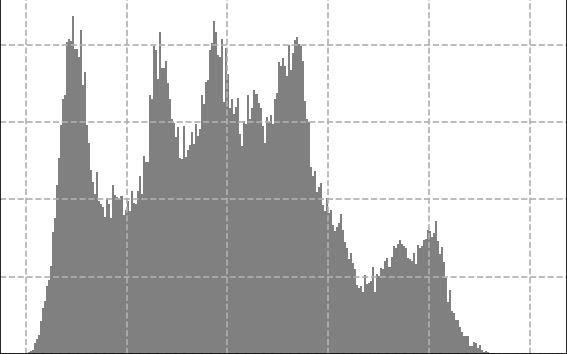
\includegraphics[width=\linewidth]{../results/lena_hist_gris}
		\captionof{figure}{Histograma original}
		\label{fig:hist_original6}
	\end{minipage}\hfill
	% Primera ecualización
	\begin{minipage}{0.32\linewidth}
		\centering
		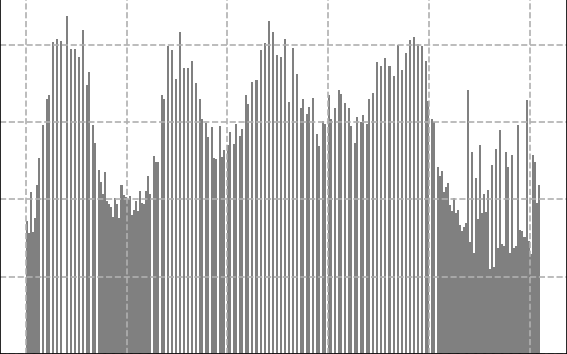
\includegraphics[width=\linewidth]{../results/lena_hist_gris_ecualizado}
		\captionof{figure}{1ª ecualización}
		\label{fig:hist_ecualizado6a}
	\end{minipage}\hfill
	% Segunda ecualización
	\begin{minipage}{0.32\linewidth}
		\centering
		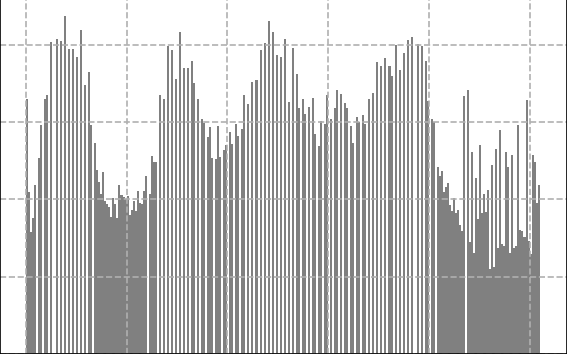
\includegraphics[width=\linewidth]{../results/lena_hist_gris_ecualizado2}
		\captionof{figure}{2ª ecualización}
		\label{fig:hist_ecualizado6b}
	\end{minipage}
\end{frame}

\begin{frame}[fragile]{Resultados - Imágenes}
	\justifying
	En la Figura~\ref{fig:lenaoriginal6} se observa la imagen original.  
	Tras la primera \textcolor{unahurverde}{\textbf{ecualización}} se obtuvo la versión de la Figura~\ref{fig:lenaej6a},  
	y al aplicar la \textcolor{unahurverde}{\textbf{ecualización}} una segunda vez se llegó a la Figura~\ref{fig:lenaej6b}.
	
	\vspace{0.5cm}
	\centering
	% Imagen original
	\begin{minipage}{0.32\linewidth}
		\centering
		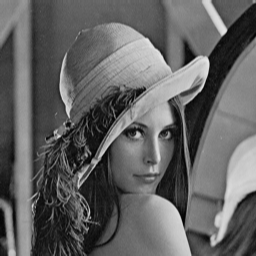
\includegraphics[width=\linewidth]{../results/lena_original}
		\captionof{figure}{Imagen original}
		\label{fig:lenaoriginal6}
	\end{minipage}\hfill
	% Imagen 1ª ecualización
	\begin{minipage}{0.32\linewidth}
		\centering
		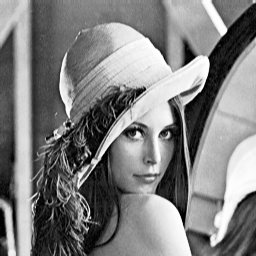
\includegraphics[width=\linewidth]{../results/lena_ej5}
		\captionof{figure}{1ª ecualización}
		\label{fig:lenaej6a}
	\end{minipage}\hfill
	% Imagen 2ª ecualización
	\begin{minipage}{0.32\linewidth}
		\centering
		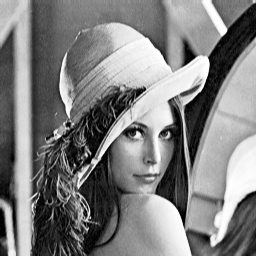
\includegraphics[width=\linewidth]{../results/lena_ej6}
		\captionof{figure}{2ª ecualización}
		\label{fig:lenaej6b}
	\end{minipage}
\end{frame}

\begin{frame}{Explicación}
	\justifying
	\footnotesize
	
	Al ecualizar el histograma de una imagen por segunda vez se pueden notar varios puntos importantes:
	
	\begin{block}{Observaciones}
		\begin{itemize}
			\item Los cambios en la distribución de niveles de gris son mínimos 
			(\textcolor{unahurverde}{imperceptibles en la imagen}).
			
			\item La primera ecualización ya redistribuyó los niveles de gris 
			de manera casi uniforme, por lo que aplicar el proceso nuevamente 
			no genera mejoras significativas en los niveles de gris.
			
			\item En otras palabras, después de la primera ecualización, 
			el histograma está bastante \textcolor{unahurverde}{“uniforme”}, y la segunda pasada simplemente mantiene esa distribución, 
			sin alterar demasiado la apariencia de la imagen.
		\end{itemize}
	\end{block}
\end{frame}


\section{Ejercicio 7}

\begin{frame}
	\begin{center}
		\textcolor{unahurverde}{\textbf{Consigna 7:}}
	\end{center}
	\justifying
	
	Implementar generadores de números aleatorios con las siguientes distribuciones:
	
	\begin{enumerate}%[label=\alph*)]
		\item Gaussiana con desviación estándar $\sigma$ y valor medio $\mu$.
		\item Rayleigh con parámetro $\xi$.
		\item Exponencial con parámetro $\lambda$.
	\end{enumerate}
	
	\vspace{0.3cm}
	
	Luego graficar los histogramas correspondientes.  
	Puede utilizarse una librería que genere números aleatorios.  
	Los parámetros del generador deben ser parámetros de entrada.
\end{frame}

\begin{frame}[fragile]{Código}
	\justifying
	Para generar los números aleatorios (1000) con las distribuciones correspondientes se realizó la siguiente función:
	
	\begin{lstlisting}[language=Python]
def _generar_vector_ruido(self, distribucion, intensidad, cantidad):
	# distribucion = np.random.normal, np.random.rayleigh, np.random.exponential
	vector_aleatorio = distribucion(scale=intensidad, size=(cantidad, 1))
	
	return vector_aleatorio
	\end{lstlisting}
	
	\vfill
	\footnotesize \textcolor{lightgray}{(*) en np.random.normal el parámetro "loc" predeterminadamente es 0.}
\end{frame}

\begin{frame}[fragile]{Resultados}
	\justifying
	A continuación se muestran los histogramas generados para distintas distribuciones: 
	Gaussiana, Rayleigh y Exponencial.
	\vspace{0.3cm}
	
	\centering
	% Primera imagen
	\begin{minipage}{0.32\linewidth}
		\centering
		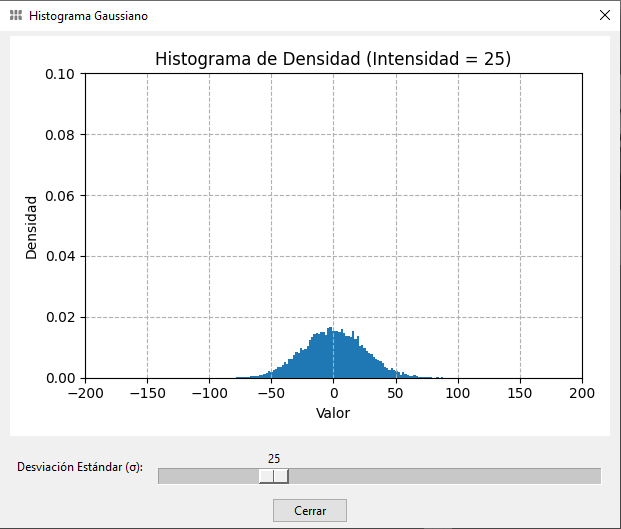
\includegraphics[width=\linewidth]{../results/dist_gauss}
		\captionof{figure}{Dist gaussiana}
	\end{minipage}\hfill
	% Segunda imagen
	\begin{minipage}{0.32\linewidth}
		\centering
		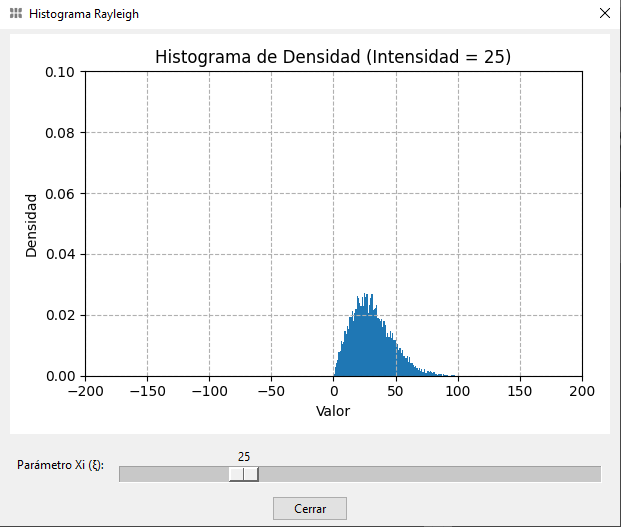
\includegraphics[width=\linewidth]{../results/dist_rayleigh}
		\captionof{figure}{Dist rayleigh}
	\end{minipage}\hfill
	% Tercera imagen
	\begin{minipage}{0.32\linewidth}
		\centering
		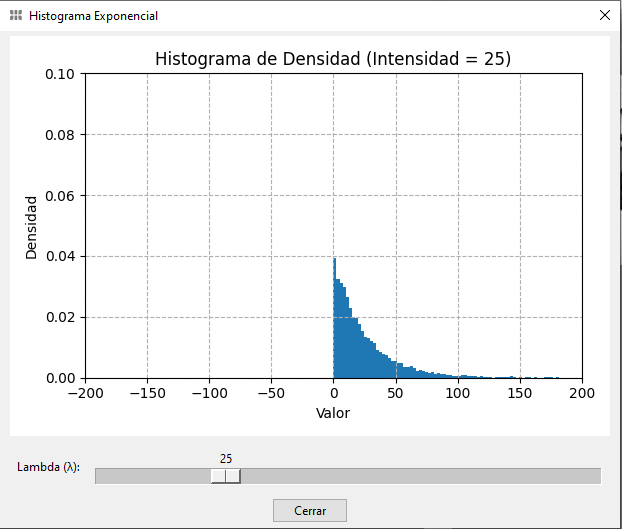
\includegraphics[width=\linewidth]{../results/dist_exponencial}
		\captionof{figure}{Dist exp}
	\end{minipage}
	
	\vfill
\footnotesize \textcolor{lightgray}{(*) Es conveniente probarlo en el programa para mayor interactividad.}
\end{frame}

\section{Ejercicio 8}

\begin{frame}
	\begin{center}
		\textcolor{unahurverde}{\textbf{Consigna 8:}}
	\end{center}
	\justifying
	
	Utilizando los generadores del punto anterior, implementar los siguientes puntos para agregar ruido a una imagen.
	
	\begin{enumerate}%[label=\alph*)]
		\item Contaminar un porcentaje de una imagen con ruido Gaussiano aditivo.
		\item Contaminar un porcentaje de una imagen con ruido Rayleigh multiplicativo.
		\item Contaminar un porcentaje de una imagen con ruido exponencial multiplicativo.
	\end{enumerate}
	
	\vspace{0.3cm}
	
	El porcentaje de contaminación y los parámetros del generador deben ser parámetros de entrada.
\end{frame}

\begin{frame}[fragile]{Agregar ruido}
	\justifying
	
	Dada una imagen $I$ de dimensión $m \times n$. La estrategia para contaminar $I$ y obtener $I_C$ la imagen contaminada es:
	
	\begin{block}{Estrategia}
		\begin{enumerate}
			\item Definir el porcentaje de contaminación d (se toma como parámetro).
			\item Elegir aleatoriamente d píxeles de la imagen y construir el conjunto $D = (i,j)$ el conjunto de píxeles seleccionados.
			\item Definir el parámetro de escala $\lambda$, $\mu$ o $\xi$ (se toma como parámetro).
			\item Generar d valores aleatorios con la distribución correspondiente (se toma como vector\_ruido).
			\item Luego en los indices $D$ de la imagen $I$ multiplicar o sumar el escalar  $k$ del vector ruido al valor del pixel según corresponda.
		\end{enumerate}
	\end{block}
\end{frame}


\begin{frame}[fragile]{Código}
	\justifying
	Para aplicar el ruido en la imagen utilizaremos la siguiente función:
	
	\begin{lstlisting}[language=Python]
def _aplicar_ruido(self, imagen, tipo, vector_ruido, d):
	imagen_np = np.array(imagen).astype(float)
	m, n, _ = imagen_np.shape
	
	# Cantidad de píxeles contaminados
	num_contaminados = int((d * (m * n)) / 100)
	# Indices (i, j) de los píxeles contaminados
	D = np.unravel_index(np.random.choice(m * n, num_contaminados, replace=False),(m, n))
	
	if tipo == "Aditivo": imagen_np[D] += vector_ruido
	elif tipo == "Multiplicativo": imagen_np[D] *= vector_ruido
	
	resultado_np = self._escalar_255(imagen_np)
	self.imagen_procesada = Image.fromarray(resultado_np)
	\end{lstlisting}
	
	\vfill
	\footnotesize \textcolor{lightgray}{(*) np.random.choice (ver \cite{numpy.random.choice}). np.unravel\_index (ver \cite{numpy.unravel_index}).}
\end{frame}

\begin{frame}[fragile]{Resultados}
	\justifying
	Al contaminar la imagen con \textcolor{unahurverde}{\textbf{ruido gaussiano aditivo}} y $\sigma=20$, 
	se obtuvo el resultado que se muestra en la Figura~\ref{fig:lenaej8a}.
	\vspace{0.5cm}
	
	\centering
	\begin{minipage}{0.45\linewidth}
		\centering
		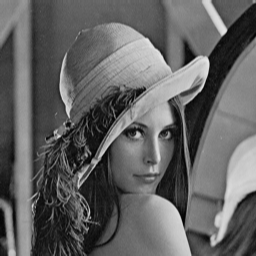
\includegraphics[width=\linewidth]{../results/lena_original}
		\captionof{figure}{Imagen original}
		\label{fig:lenaoriginal8a}
	\end{minipage}\hfill
	\begin{minipage}{0.45\linewidth}
		\centering
		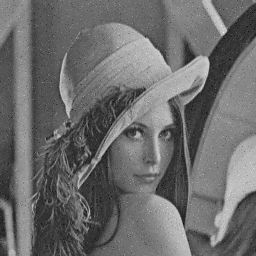
\includegraphics[width=\linewidth]{../results/lena_ej8a}
		\captionof{figure}{Imagen con ruido}
		\label{fig:lenaej8a}
	\end{minipage}
\end{frame}

\begin{frame}[fragile]{Resultados}
	\justifying
	Al contaminar la imagen con \textcolor{unahurverde}{\textbf{ruido Rayleigh multiplicativo}} y $\xi=2$, 
	se obtuvo el resultado que se observa en la Figura~\ref{fig:lenaej8b}.
	
	\vspace{0.5cm}
	\centering
	\begin{minipage}{0.45\linewidth}
		\centering
		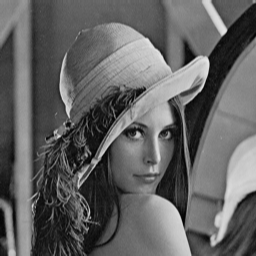
\includegraphics[width=\linewidth]{../results/lena_original}
		\captionof{figure}{Imagen original}
		\label{fig:lenaoriginal8b}
	\end{minipage}\hfill
	\begin{minipage}{0.45\linewidth}
		\centering
		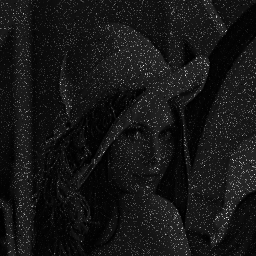
\includegraphics[width=\linewidth]{../results/lena_ej8b}
		\captionof{figure}{Imagen con ruido}
		\label{fig:lenaej8b}
	\end{minipage}
\end{frame}

\begin{frame}[fragile]{Resultados}
	\justifying
	Al contaminar la imagen con \textcolor{unahurverde}{\textbf{ruido exponencial multiplicativo}} y $\frac{1}{\lambda}=1$, 
	se obtuvo la versión que aparece en la Figura~\ref{fig:lenaej8c}.
	
	\vspace{0.5cm}
	\centering
	\begin{minipage}{0.45\linewidth}
		\centering
		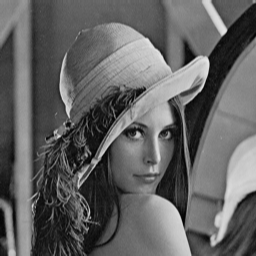
\includegraphics[width=\linewidth]{../results/lena_original}
		\captionof{figure}{Imagen original}
		\label{fig:lenaoriginal8c}
	\end{minipage}\hfill
	\begin{minipage}{0.45\linewidth}
		\centering
		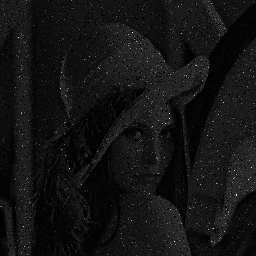
\includegraphics[width=\linewidth]{../results/lena_ej8c}
		\captionof{figure}{Imagen con ruido}
		\label{fig:lenaej8c}
	\end{minipage}
\end{frame}

\section{Ejercicio 9}

\begin{frame}
	\begin{center}
		\textcolor{unahurverde}{\textbf{Consigna 9:}}
	\end{center}
	\justifying
	
	Implementar un generador de ruido Sal y Pimienta de densidad variable, aplicarlo una
	imagen.
\end{frame}

\begin{frame}[fragile]{Ruido Sal y Pimienta}
	\justifying
	
	\begin{block}{Definición}
		Dada una imagen $I$.
		\begin{itemize}
			\item Elegir $p \in (0, 0,5)$
			\item Recorrer cada pixel $(i, j)$ de $I$.
			\begin{itemize}
				\item Tomar $x \sim U(0,1)$
				\item Si $x \leq p$ entonces $I(i,j) = 0$
				\item Si $x > 1 - p$ entonces $I(i,j) = 255$
			\end{itemize}
		\end{itemize}
	\end{block}
\end{frame}

\begin{frame}[fragile]{Código}
	\justifying
	
	\begin{lstlisting}[language=Python]
def _aplicar_ruido_sal_y_pimienta(self, imagen, p):
	imagen_np = np.array(imagen.convert('RGB'))
	
	m, n, _ = imagen_np.shape
	
	for i in range(m):
		for j in range(n):
			x = np.random.rand()
			if x <= p:
				imagen_np[i, j, :] = 0 # pimienta (negro)
			elif x > (1-p):
				imagen_np[i, j, :] = 255 # sal (blanco)
	
	self.imagen_procesada = Image.fromarray(imagen_np)
	\end{lstlisting}
	
	\vfill
	\footnotesize \textcolor{lightgray}{(*) Aunque en el slider uno pone la probabilidad, a la función le llega p = (porcentaje / 2) / 100.}
\end{frame}

\begin{frame}[fragile]{Resultados}
	\justifying
	Al aplicar \textcolor{unahurverde}{\textbf{ruido Sal y Pimienta}} a una imagen con probabilidad = 10 sobre la Figura~\ref{fig:lenaoriginal9},  
	se obtuvo la versión ruidosa que aparece en la Figura~\ref{fig:lenaej9}.
	\vspace{0.5cm}
	
	\centering
	\begin{minipage}{0.45\linewidth}
		\centering
		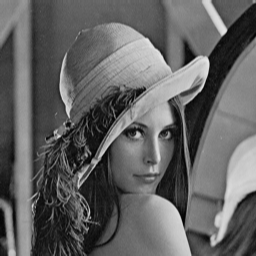
\includegraphics[width=\linewidth]{../results/lena_original}
		\captionof{figure}{Imagen original}
		\label{fig:lenaoriginal9}
	\end{minipage}\hfill
	\begin{minipage}{0.45\linewidth}
		\centering
		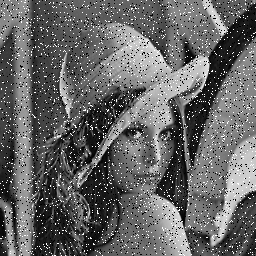
\includegraphics[width=\linewidth]{../results/lena_ej9}
		\captionof{figure}{Imagen con ruido}
		\label{fig:lenaej9}
	\end{minipage}
\end{frame}

\section{Ejercicio 10}

\begin{frame}
	\begin{center}
		\textcolor{unahurverde}{\textbf{Consigna 10:}}
	\end{center}
	\justifying
	
	Implementar una ventana deslizante que pueda aplicarse a una imagen con máscaras de
	tamaño variable, cuadrada y aplicar a una imagen las siguientes máscaras:

	\begin{enumerate}
		\item Filtro de la media.
		\item Filtro de la mediana.
		\item Filtro de la mediana ponderada.
		\item Filtro de Gauss para diferentes valores de $\sigma$ y $\mu = 0$.
		\item Realce de Bordes.
	\end{enumerate}
\end{frame}

\begin{frame}[fragile]{Aplicación de filtros}
	\justifying
	
	\begin{block}{Estrategia}
		\begin{enumerate}
			\item Transformar la imagen a un \texttt{np.array} en formato \texttt{RGB}.
			\item Obtener sus dimensiones $(m, n, c)$.
			\item Calcular las dimensiones del filtro $(k, l)$ y el \textit{padding} necesario.
			\item Generar una versión \textit{padded} de la imagen.
			\item Inicializar una matriz vacía para la imagen filtrada.
			\item Recorrer cada píxel y canal de color:
			\begin{itemize}
				\item Extraer la región correspondiente al filtro.
				\item Multiplicar y sumar con la máscara del filtro.
				\item Escalar el valor por el factor definido.
			\end{itemize}
			\item Escalar el resultado al rango $[0, 255]$.
			\item Convertir el resultado nuevamente a imagen.
		\end{enumerate}
	\end{block}
\end{frame}

\begin{frame}[fragile]{Código - Aplicar filtro}
	\justifying
	
	\begin{lstlisting}[language=Python]
def _aplicar_filtro(self, imagen, filtro, factor):
	imagen_np = np.array(imagen.convert('RGB')).astype(float)
	m, n, _ = imagen_np.shape
	k, l = filtro.shape
	pad_h, pad_w = k//2, l//2
	
	imagen_padded = np.pad(imagen_np, ((pad_h, pad_h), (pad_w, pad_w), (0, 0)), mode='constant')
	imagen_filtrada = np.zeros_like(imagen_np)
	
	for i in range(m):
		for j in range(n):
			for c in range(3):
				region = imagen_padded[i:i+k, j:j+l, c]
				valor = np.sum(region * filtro) * factor
				imagen_filtrada[i, j, c] = valor
	
	resultado_np = self._escalar_255(imagen_filtrada)
	self.imagen_procesada = Image.fromarray(resultado_np)
	\end{lstlisting}
\end{frame}

\begin{frame}[fragile]{Filtro de la media}
	\justifying
	El filtro de la media se obtiene de la siguiente manera:
	
	\begin{lstlisting}[language=Python]
def _filtro_media(self, k):
	filtro = np.ones((k, k))
	
	factor = 1 / np.sum(filtro)
	return (filtro, factor)
	\end{lstlisting}
	
	\vfill
	\footnotesize \textcolor{lightgray}{(*) np.pad (ver \cite{numpy.pad}).}\\
	\footnotesize \textcolor{lightgray}{(*) np.repeat (ver \cite{numpy.repeat}).}
\end{frame}

\begin{frame}[fragile]{Resultados - Filtro Media}
	\justifying
	Al aplicar \textcolor{unahurverde}{\textbf{el filtro Media}} sobre la imagen de la Figura~\ref{fig:lenaoriginal10a} con $k=3$,  
	se obtuvo la versión suavizada que aparece en la Figura~\ref{fig:lenaej10a}.
	
	\vspace{0.5cm}
	\centering
	\begin{minipage}{0.45\linewidth}
		\centering
		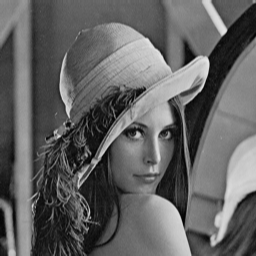
\includegraphics[width=\linewidth]{../results/lena_original}
		\captionof{figure}{Imagen original}
		\label{fig:lenaoriginal10a}
	\end{minipage}\hfill
	\begin{minipage}{0.45\linewidth}
		\centering
		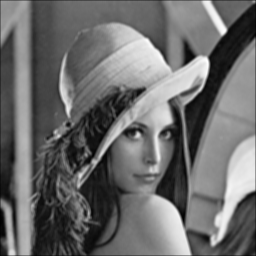
\includegraphics[width=\linewidth]{../results/lena_ej10a}
		\captionof{figure}{Imagen con filtro Media}
		\label{fig:lenaej10a}
	\end{minipage}
\end{frame}

\begin{frame}[fragile]{Código - Aplicar filtro Mediana}
	\justifying
	
	\begin{lstlisting}[language=Python]
def _aplicar_filtro_mediana(self, imagen, filtro):
	imagen_np = np.array(imagen.convert('RGB')).astype(float)
	m, n, _ = imagen_np.shape
	k, l = filtro.shape
	pad_h, pad_w = k//2, l//2
	imagen_padded = np.pad(imagen_np, ((pad_h, pad_h), (pad_w, pad_w), (0, 0)), mode='constant')
	imagen_filtrada = np.zeros_like(imagen_np)
	indices_repeticion = filtro.flatten().astype(int)
	
	for i in range(m):
		for j in range(n):
			for c in range(3):
				region = imagen_padded[i:i+k, j:j+l, c]
				valores = np.repeat(region.flatten(), indices_repeticion) # Indica rep de cada indice
				mediana = np.median(valores)
				imagen_filtrada[i, j, c] = mediana
	self.imagen_procesada = Image.fromarray(imagen_filtrada.astype(np.uint8))
	\end{lstlisting}
\end{frame}

\begin{frame}[fragile]{Resultados - Filtro Mediana}
	\justifying
	Al aplicar \textcolor{unahurverde}{\textbf{el filtro Mediana}} sobre la imagen de la Figura~\ref{fig:lenaoriginal10b} con $k=3$,  
	se obtuvo la versión suavizada que aparece en la Figura~\ref{fig:lenaej10b}.
	
	\vspace{0.5cm}
	\centering
	\begin{minipage}{0.45\linewidth}
		\centering
		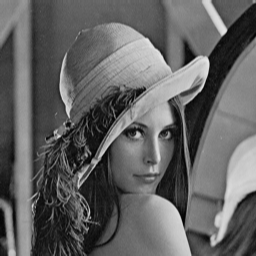
\includegraphics[width=\linewidth]{../results/lena_original}
		\captionof{figure}{Imagen original}
		\label{fig:lenaoriginal10b}
	\end{minipage}\hfill
	\begin{minipage}{0.45\linewidth}
		\centering
		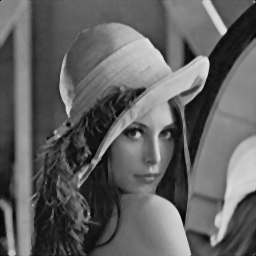
\includegraphics[width=\linewidth]{../results/lena_ej10b}
		\captionof{figure}{Imagen con filtro Mediana}
		\label{fig:lenaej10b}
	\end{minipage}
\end{frame}

\begin{frame}[fragile]{Filtro Mediana Ponderada}
	\justifying
	
	\begin{lstlisting}[language=Python]
def _filtro_mediana_ponderada(self, k):
	filtro_gauss, _ = self._filtro_gaussiano(k)
	filtro = (filtro_gauss * 50).astype(int)
	
	factor = 1
	return (filtro, factor)
	\end{lstlisting}
\end{frame}

\begin{frame}[fragile]{Resultados - Filtro Mediana Ponderada}
	\justifying
	Al aplicar \textcolor{unahurverde}{\textbf{el filtro Mediana Ponderada}} sobre la imagen de la Figura~\ref{fig:lenaoriginal10c} con $k=3$,  
	se obtuvo la versión suavizada que aparece en la Figura~\ref{fig:lenaej10c}.
	
	\vspace{0.5cm}
	\centering
	\begin{minipage}{0.45\linewidth}
		\centering
		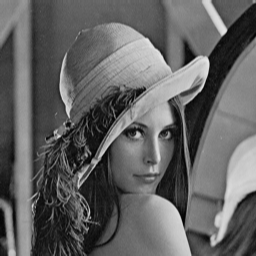
\includegraphics[width=\linewidth]{../results/lena_original}
		\captionof{figure}{Imagen original}
		\label{fig:lenaoriginal10c}
	\end{minipage}\hfill
	\begin{minipage}{0.45\linewidth}
		\centering
		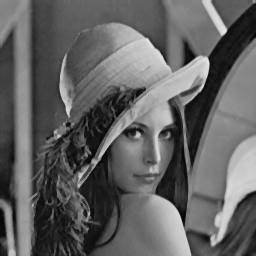
\includegraphics[width=\linewidth]{../results/lena_ej10c}
		\captionof{figure}{Imagen con filtro Mediana Ponderada}
		\label{fig:lenaej10c}
	\end{minipage}
\end{frame}

\begin{frame}[fragile]{Filtro Gaussiano}
	\justifying
	
	\begin{lstlisting}[language=Python]
		def _filtro_gaussiano(self, k):
		filtro = np.ones((k, k)).astype(float)
		u = k // 2 # Centro donde el valor debe ser máximo (son iguales ya que es cuadrada)
		sigma = (k-1) / 2
		
		for x in range(k):
		for y in range(k):
		filtro[x, y] = (1 / (2 * np.pi * sigma**2)) * np.exp(-((x - u)**2 + (y - u)**2)/(2 * sigma**2))
		
		factor = 1 / np.sum(filtro)
		return (filtro, factor)
	\end{lstlisting}
\end{frame}

\begin{frame}[fragile]{Resultados - Filtro Gaussiano}
	\justifying
	Al aplicar \textcolor{unahurverde}{\textbf{el filtro Gaussiano}} sobre la imagen de la Figura~\ref{fig:lenaoriginal10d},  
	se obtuvieron las versiones suavizadas con distintos valores de sigma, que se muestran en las Figuras~\ref{fig:lenaej10d1} y~\ref{fig:lenaej10d2}.
	
	\vspace{0.5cm}
	\centering
	% Imagen original
	\begin{minipage}{0.32\linewidth}
		\centering
		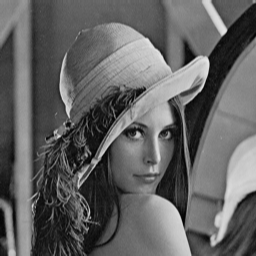
\includegraphics[width=\linewidth]{../results/lena_original}
		\captionof{figure}{Imagen original}
		\label{fig:lenaoriginal10d}
	\end{minipage}\hfill
	% Sigma = 1
	\begin{minipage}{0.32\linewidth}
		\centering
		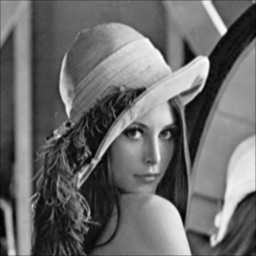
\includegraphics[width=\linewidth]{../results/lena_ej10d1}
		\captionof{figure}{Filtro Gaussiano, $\sigma = 1$}
		\label{fig:lenaej10d1}
	\end{minipage}\hfill
	% Sigma = 2
	\begin{minipage}{0.32\linewidth}
		\centering
		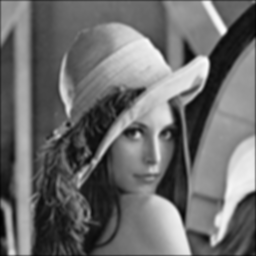
\includegraphics[width=\linewidth]{../results/lena_ej10d2}
		\captionof{figure}{Filtro Gaussiano, $\sigma = 2$}
		\label{fig:lenaej10d2}
	\end{minipage}
\end{frame}


\begin{frame}[fragile]{Filtro Realce de Bordes}
	\justifying
	
	\begin{lstlisting}[language=Python]
def _filtro_realce(self, k):
	filtro = -1 * np.ones((k, k))
	filtro[k//2, k//2] = k**2 - 1
	
	factor = 1
	return (filtro, factor)
	\end{lstlisting}
\end{frame}

\begin{frame}[fragile]{Resultados - Filtro Realce de Bordes}
	\justifying
	Al aplicar \textcolor{unahurverde}{\textbf{el filtro Realce de Bordes}} sobre la imagen de la Figura~\ref{fig:lenaoriginal10e},  
	se obtuvo la versión resaltada que aparece en la Figura~\ref{fig:lenaej10e}.
	
	\vspace{0.5cm}
	\centering
	\begin{minipage}{0.45\linewidth}
		\centering
		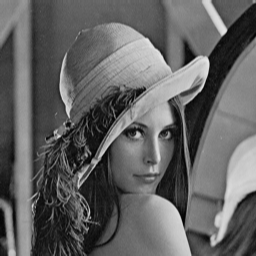
\includegraphics[width=\linewidth]{../results/lena_original}
		\captionof{figure}{Imagen original}
		\label{fig:lenaoriginal10e}
	\end{minipage}\hfill
	\begin{minipage}{0.45\linewidth}
		\centering
		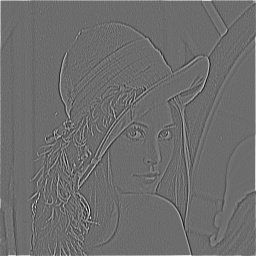
\includegraphics[width=\linewidth]{../results/lena_ej10e}
		\captionof{figure}{Imagen con filtro Realce de Bordes}
		\label{fig:lenaej10e}
	\end{minipage}
\end{frame}

\section{Ejercicio 11}

\begin{frame}
	\begin{center}
		\textcolor{unahurverde}{\textbf{Consigna 11:}}
	\end{center}
	\justifying
	
	Repetir el punto anterior aplicándolo a las mismas imágenes contaminadas con:
	
	\begin{enumerate}
		\item Ruido Gaussiano aditivo para varios de $\sigma$ y $\mu = 0$.
		\item Ruido Rayleigh multiplicativo para varios valores de $\xi$. 
	\end{enumerate}
\end{frame}

\subsection{Punto a}

\begin{frame}[fragile]{Filtro Media sobre Ruido Gaussiano}
	\justifying
	\footnotesize
	Se aplicó \textcolor{unahurverde}{\textbf{el filtro Media}} sobre imágenes contaminadas con \textcolor{unahurverde}{\textbf{ruido Gaussiano aditivo}}  
	con $\mu = 0$ y distintos valores de $\sigma$ (10, 20 y 50).  
	La fila superior muestra las imágenes con ruido y la fila inferior los resultados tras aplicar el filtro con $k=3$.
	
	\centering
	% Primera fila: imágenes con ruido
	\begin{minipage}{0.25\linewidth}
		\centering
		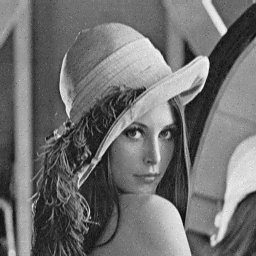
\includegraphics[width=\linewidth]{../results/lena_gauss_sigma10}
	\end{minipage}\hfill
	\begin{minipage}{0.25\linewidth}
		\centering
		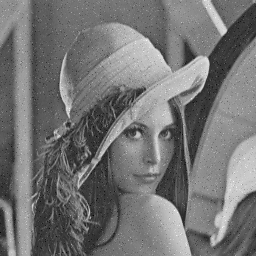
\includegraphics[width=\linewidth]{../results/lena_gauss_sigma20}
	\end{minipage}\hfill
	\begin{minipage}{0.25\linewidth}
		\centering
		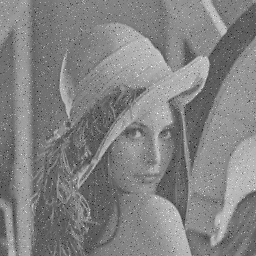
\includegraphics[width=\linewidth]{../results/lena_gauss_sigma50}
	\end{minipage}
	
	% Segunda fila: imágenes filtradas
	\begin{minipage}{0.25\linewidth}
		\centering
		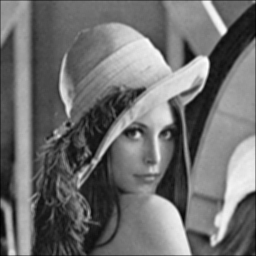
\includegraphics[width=\linewidth]{../results/lena_gauss_sigma10_media}
	\end{minipage}\hfill
	\begin{minipage}{0.25\linewidth}
		\centering
		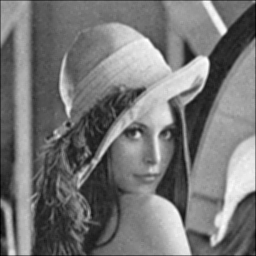
\includegraphics[width=\linewidth]{../results/lena_gauss_sigma20_media}
	\end{minipage}\hfill
	\begin{minipage}{0.25\linewidth}
		\centering
		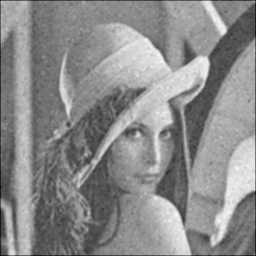
\includegraphics[width=\linewidth]{../results/lena_gauss_sigma50_media}
	\end{minipage}
\end{frame}

\begin{frame}[fragile]{Filtro Mediana sobre Ruido Gaussiano}
	\justifying
	\footnotesize
	Se aplicó \textcolor{unahurverde}{\textbf{el filtro Mediana}} sobre imágenes contaminadas con \textcolor{unahurverde}{\textbf{ruido Gaussiano aditivo}}  
	con $\mu = 0$ y distintos valores de $\sigma$ (10, 20 y 50).  
	La fila superior muestra las imágenes con ruido y la fila inferior los resultados tras aplicar el filtro.
	
	\centering
	% Primera fila: imágenes con ruido
	\begin{minipage}{0.25\linewidth}
		\centering
		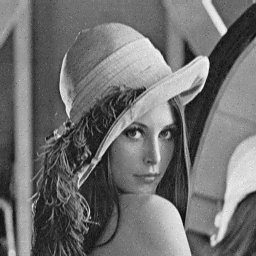
\includegraphics[width=\linewidth]{../results/lena_gauss_sigma10}
	\end{minipage}\hfill
	\begin{minipage}{0.25\linewidth}
		\centering
		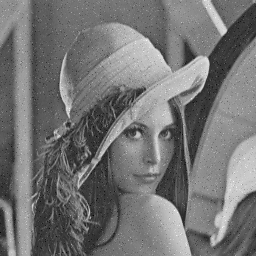
\includegraphics[width=\linewidth]{../results/lena_gauss_sigma20}
	\end{minipage}\hfill
	\begin{minipage}{0.25\linewidth}
		\centering
		\includegraphics[width=\linewidth]{../results/lena_gauss_sigma50}
	\end{minipage}
	
	% Segunda fila: imágenes filtradas
	\begin{minipage}{0.25\linewidth}
		\centering
		\includegraphics[width=\linewidth]{../results/lena_gauss_sigma10_mediana}
	\end{minipage}\hfill
	\begin{minipage}{0.25\linewidth}
		\centering
		\includegraphics[width=\linewidth]{../results/lena_gauss_sigma20_mediana}
	\end{minipage}\hfill
	\begin{minipage}{0.25\linewidth}
		\centering
		\includegraphics[width=\linewidth]{../results/lena_gauss_sigma50_mediana}
	\end{minipage}
\end{frame}

\begin{frame}[fragile]{Filtro Mediana Ponderada sobre Ruido Gaussiano}
	\justifying
	\footnotesize
	Se aplicó \textcolor{unahurverde}{\textbf{el filtro Mediana Ponderada}} sobre imágenes contaminadas con \textcolor{unahurverde}{\textbf{ruido Gaussiano aditivo}}  
	con $\mu = 0$ y distintos valores de $\sigma$ (10, 20 y 50).  
	La fila superior muestra las imágenes con ruido y la fila inferior los resultados tras aplicar el filtro.
	
	\centering
	% Primera fila: imágenes con ruido
	\begin{minipage}{0.25\linewidth}
		\centering
		\includegraphics[width=\linewidth]{../results/lena_gauss_sigma10}
	\end{minipage}\hfill
	\begin{minipage}{0.25\linewidth}
		\centering
		\includegraphics[width=\linewidth]{../results/lena_gauss_sigma20}
	\end{minipage}\hfill
	\begin{minipage}{0.25\linewidth}
		\centering
		\includegraphics[width=\linewidth]{../results/lena_gauss_sigma50}
	\end{minipage}
	
	% Segunda fila: imágenes filtradas
	\begin{minipage}{0.25\linewidth}
		\centering
		\includegraphics[width=\linewidth]{../results/lena_gauss_sigma10_mediana_ponderada}
	\end{minipage}\hfill
	\begin{minipage}{0.25\linewidth}
		\centering
		\includegraphics[width=\linewidth]{../results/lena_gauss_sigma20_mediana_ponderada}
	\end{minipage}\hfill
	\begin{minipage}{0.25\linewidth}
		\centering
		\includegraphics[width=\linewidth]{../results/lena_gauss_sigma50_mediana_ponderada}
	\end{minipage}
\end{frame}

\begin{frame}[fragile]{Filtro Gaussiano sobre Ruido Gaussiano}
	\justifying
	\footnotesize
	Se aplicó \textcolor{unahurverde}{\textbf{el filtro Gaussiano}} sobre imágenes contaminadas con \textcolor{unahurverde}{\textbf{ruido Gaussiano aditivo}}  
	con $\mu = 0$ y distintos valores de $\sigma$ (10, 20 y 50).  
	La fila superior muestra las imágenes con ruido y la fila inferior los resultados tras aplicar el filtro.
	
	\centering
	% Primera fila: imágenes con ruido
	\begin{minipage}{0.25\linewidth}
		\centering
		\includegraphics[width=\linewidth]{../results/lena_gauss_sigma10}
	\end{minipage}\hfill
	\begin{minipage}{0.25\linewidth}
		\centering
		\includegraphics[width=\linewidth]{../results/lena_gauss_sigma20}
	\end{minipage}\hfill
	\begin{minipage}{0.25\linewidth}
		\centering
		\includegraphics[width=\linewidth]{../results/lena_gauss_sigma50}
	\end{minipage}
	
	% Segunda fila: imágenes filtradas
	\begin{minipage}{0.25\linewidth}
		\centering
		\includegraphics[width=\linewidth]{../results/lena_gauss_sigma10_gaussiano}
	\end{minipage}\hfill
	\begin{minipage}{0.25\linewidth}
		\centering
		\includegraphics[width=\linewidth]{../results/lena_gauss_sigma20_gaussiano}
	\end{minipage}\hfill
	\begin{minipage}{0.25\linewidth}
		\centering
		\includegraphics[width=\linewidth]{../results/lena_gauss_sigma50_gaussiano}
	\end{minipage}
\end{frame}

\begin{frame}[fragile]{Filtro Realce de Bordes sobre Ruido Gaussiano}
	\justifying
	\footnotesize
	Se aplicó \textcolor{unahurverde}{\textbf{el filtro de Realce de Bordes}} sobre imágenes contaminadas con \textcolor{unahurverde}{\textbf{ruido Gaussiano aditivo}}  
	con $\mu = 0$ y distintos valores de $\sigma$ (10, 20 y 50).  
	La fila superior muestra las imágenes con ruido y la fila inferior los resultados tras aplicar el filtro.
	
	\centering
	% Primera fila: imágenes con ruido
	\begin{minipage}{0.25\linewidth}
		\centering
		\includegraphics[width=\linewidth]{../results/lena_gauss_sigma10}
	\end{minipage}\hfill
	\begin{minipage}{0.25\linewidth}
		\centering
		\includegraphics[width=\linewidth]{../results/lena_gauss_sigma20}
	\end{minipage}\hfill
	\begin{minipage}{0.25\linewidth}
		\centering
		\includegraphics[width=\linewidth]{../results/lena_gauss_sigma50}
	\end{minipage}
	
	% Segunda fila: imágenes filtradas
	\begin{minipage}{0.25\linewidth}
		\centering
		\includegraphics[width=\linewidth]{../results/lena_gauss_sigma10_bordes}
	\end{minipage}\hfill
	\begin{minipage}{0.25\linewidth}
		\centering
		\includegraphics[width=\linewidth]{../results/lena_gauss_sigma20_bordes}
	\end{minipage}\hfill
	\begin{minipage}{0.25\linewidth}
		\centering
		\includegraphics[width=\linewidth]{../results/lena_gauss_sigma50_bordes}
	\end{minipage}
\end{frame}

\subsection{Punto b}

\begin{frame}[fragile]{Filtro Media sobre Ruido Rayleigh}
	\justifying
	\footnotesize
	Se aplicó \textcolor{unahurverde}{\textbf{el filtro Media}} sobre imágenes contaminadas con \textcolor{unahurverde}{\textbf{ruido Rayleigh multiplicativo}}  
	con distintos valores de $\xi$ (1, 2 y 10).  
	La fila superior muestra las imágenes con ruido y la fila inferior los resultados tras aplicar el filtro con $k=3$.
	
	\centering
	% Primera fila: imágenes con ruido
	\begin{minipage}{0.25\linewidth}
		\centering
		\includegraphics[width=\linewidth]{../results/lena_rayleigh_xi1}
	\end{minipage}\hfill
	\begin{minipage}{0.25\linewidth}
		\centering
		\includegraphics[width=\linewidth]{../results/lena_rayleigh_xi2}
	\end{minipage}\hfill
	\begin{minipage}{0.25\linewidth}
		\centering
		\includegraphics[width=\linewidth]{../results/lena_rayleigh_xi10}
	\end{minipage}
	
	% Segunda fila: imágenes filtradas
	\begin{minipage}{0.25\linewidth}
		\centering
		\includegraphics[width=\linewidth]{../results/lena_rayleigh_xi1_media}
	\end{minipage}\hfill
	\begin{minipage}{0.25\linewidth}
		\centering
		\includegraphics[width=\linewidth]{../results/lena_rayleigh_xi2_media}
	\end{minipage}\hfill
	\begin{minipage}{0.25\linewidth}
		\centering
		\includegraphics[width=\linewidth]{../results/lena_rayleigh_xi10_media}
	\end{minipage}
\end{frame}

\begin{frame}[fragile]{Filtro Mediana sobre Ruido Rayleigh}
	\justifying
	\footnotesize
	Se aplicó \textcolor{unahurverde}{\textbf{el filtro Mediana}} sobre imágenes contaminadas con \textcolor{unahurverde}{\textbf{ruido Rayleigh multiplicativo}}  
	con distintos valores de $\xi$ (1, 2 y 10).  
	La fila superior muestra las imágenes con ruido y la fila inferior los resultados tras aplicar el filtro.
	
	\centering
	% Primera fila: imágenes con ruido
	\begin{minipage}{0.25\linewidth}
		\centering
		\includegraphics[width=\linewidth]{../results/lena_rayleigh_xi1}
	\end{minipage}\hfill
	\begin{minipage}{0.25\linewidth}
		\centering
		\includegraphics[width=\linewidth]{../results/lena_rayleigh_xi2}
	\end{minipage}\hfill
	\begin{minipage}{0.25\linewidth}
		\centering
		\includegraphics[width=\linewidth]{../results/lena_rayleigh_xi10}
	\end{minipage}
	
	% Segunda fila: imágenes filtradas
	\begin{minipage}{0.25\linewidth}
		\centering
		\includegraphics[width=\linewidth]{../results/lena_rayleigh_xi1_mediana}
	\end{minipage}\hfill
	\begin{minipage}{0.25\linewidth}
		\centering
		\includegraphics[width=\linewidth]{../results/lena_rayleigh_xi2_mediana}
	\end{minipage}\hfill
	\begin{minipage}{0.25\linewidth}
		\centering
		\includegraphics[width=\linewidth]{../results/lena_rayleigh_xi10_mediana}
	\end{minipage}
\end{frame}

\begin{frame}[fragile]{Filtro Mediana Ponderada sobre Ruido Rayleigh}
	\justifying
	\footnotesize
	Se aplicó \textcolor{unahurverde}{\textbf{el filtro Mediana Ponderada}} sobre imágenes contaminadas con \textcolor{unahurverde}{\textbf{ruido Rayleigh multiplicativo}}  
	con distintos valores de $\xi$ (1, 2 y 10).  
	La fila superior muestra las imágenes con ruido y la fila inferior los resultados tras aplicar el filtro.
	
	\centering
	% Primera fila: imágenes con ruido
	\begin{minipage}{0.25\linewidth}
		\centering
		\includegraphics[width=\linewidth]{../results/lena_rayleigh_xi1}
	\end{minipage}\hfill
	\begin{minipage}{0.25\linewidth}
		\centering
		\includegraphics[width=\linewidth]{../results/lena_rayleigh_xi2}
	\end{minipage}\hfill
	\begin{minipage}{0.25\linewidth}
		\centering
		\includegraphics[width=\linewidth]{../results/lena_rayleigh_xi10}
	\end{minipage}
	
	% Segunda fila: imágenes filtradas
	\begin{minipage}{0.25\linewidth}
		\centering
		\includegraphics[width=\linewidth]{../results/lena_rayleigh_xi1_mediana_ponderada}
	\end{minipage}\hfill
	\begin{minipage}{0.25\linewidth}
		\centering
		\includegraphics[width=\linewidth]{../results/lena_rayleigh_xi2_mediana_ponderada}
	\end{minipage}\hfill
	\begin{minipage}{0.25\linewidth}
		\centering
		\includegraphics[width=\linewidth]{../results/lena_rayleigh_xi10_mediana_ponderada}
	\end{minipage}
\end{frame}

\begin{frame}[fragile]{Filtro Gaussiano sobre Ruido Rayleigh}
	\justifying
	\footnotesize
	Se aplicó \textcolor{unahurverde}{\textbf{el filtro Gaussiano}} sobre imágenes contaminadas con \textcolor{unahurverde}{\textbf{ruido Rayleigh multiplicativo}}  
	con distintos valores de $\xi$ (1, 2 y 10).  
	La fila superior muestra las imágenes con ruido y la fila inferior los resultados tras aplicar el filtro.
	
	\centering
	% Primera fila: imágenes con ruido
	\begin{minipage}{0.25\linewidth}
		\centering
		\includegraphics[width=\linewidth]{../results/lena_rayleigh_xi1}
	\end{minipage}\hfill
	\begin{minipage}{0.25\linewidth}
		\centering
		\includegraphics[width=\linewidth]{../results/lena_rayleigh_xi2}
	\end{minipage}\hfill
	\begin{minipage}{0.25\linewidth}
		\centering
		\includegraphics[width=\linewidth]{../results/lena_rayleigh_xi10}
	\end{minipage}
	
	% Segunda fila: imágenes filtradas
	\begin{minipage}{0.25\linewidth}
		\centering
		\includegraphics[width=\linewidth]{../results/lena_rayleigh_xi1_gaussiano}
	\end{minipage}\hfill
	\begin{minipage}{0.25\linewidth}
		\centering
		\includegraphics[width=\linewidth]{../results/lena_rayleigh_xi2_gaussiano}
	\end{minipage}\hfill
	\begin{minipage}{0.25\linewidth}
		\centering
		\includegraphics[width=\linewidth]{../results/lena_rayleigh_xi10_gaussiano}
	\end{minipage}
\end{frame}

\begin{frame}[fragile]{Filtro Realce de Bordes sobre Ruido Rayleigh}
	\justifying
	\footnotesize
	Se aplicó \textcolor{unahurverde}{\textbf{el filtro de Realce de Bordes}} sobre imágenes contaminadas con \textcolor{unahurverde}{\textbf{ruido Rayleigh multiplicativo}}  
	con distintos valores de $\xi$ (1, 2 y 10).  
	La fila superior muestra las imágenes con ruido y la fila inferior los resultados tras aplicar el filtro.
	
	\centering
	% Primera fila: imágenes con ruido
	\begin{minipage}{0.25\linewidth}
		\centering
		\includegraphics[width=\linewidth]{../results/lena_rayleigh_xi1}
	\end{minipage}\hfill
	\begin{minipage}{0.25\linewidth}
		\centering
		\includegraphics[width=\linewidth]{../results/lena_rayleigh_xi2}
	\end{minipage}\hfill
	\begin{minipage}{0.25\linewidth}
		\centering
		\includegraphics[width=\linewidth]{../results/lena_rayleigh_xi10}
	\end{minipage}
	
	% Segunda fila: imágenes filtradas
	\begin{minipage}{0.25\linewidth}
		\centering
		\includegraphics[width=\linewidth]{../results/lena_rayleigh_xi1_bordes}
	\end{minipage}\hfill
	\begin{minipage}{0.25\linewidth}
		\centering
		\includegraphics[width=\linewidth]{../results/lena_rayleigh_xi2_bordes}
	\end{minipage}\hfill
	\begin{minipage}{0.25\linewidth}
		\centering
		\includegraphics[width=\linewidth]{../results/lena_rayleigh_xi10_bordes}
	\end{minipage}
\end{frame}


\section{Ejercicio 12}

\begin{frame}
	\begin{center}
		\textcolor{unahurverde}{\textbf{Consigna 12:}}
	\end{center}
	\justifying
	
	 Contaminar con ruido Sal y Pimienta con diferentes densidades y aplicarle el filtro de la media y de la mediana. Observar los resultados.
\end{frame}

\begin{frame}[fragile]{Resultados - Filtros sobre ruido Sal y Pimienta (a)}
	\justifying
	Sobre la imagen contaminada con \textcolor{unahurverde}{\textbf{ruido Sal y Pimienta}} con $p=0.01$ (Figura~\ref{fig:lenaej12a})  
	se aplicaron los filtros de \textcolor{unahurverde}{\textbf{Media}} con $k=5$ y \textcolor{unahurverde}{\textbf{Mediana}} con $k=3$, obteniendo las Figuras~\ref{fig:lenaej12a1} y~\ref{fig:lenaej12a2}.
	
	\vspace{0.5cm}
	\centering
	% Imagen con ruido
	\begin{minipage}{0.32\linewidth}
		\centering
		\includegraphics[width=\linewidth]{../results/lena_ej12a}
		\captionof{figure}{Imagen con ruido}
		\label{fig:lenaej12a}
	\end{minipage}\hfill
	% Filtro Media
	\begin{minipage}{0.32\linewidth}
		\centering
		\includegraphics[width=\linewidth]{../results/lena_ej12a1}
		\captionof{figure}{Filtro Media}
		\label{fig:lenaej12a1}
	\end{minipage}\hfill
	% Filtro Mediana
	\begin{minipage}{0.32\linewidth}
		\centering
		\includegraphics[width=\linewidth]{../results/lena_ej12a2}
		\captionof{figure}{Filtro Mediana}
		\label{fig:lenaej12a2}
	\end{minipage}
\end{frame}

\begin{frame}[fragile]{Resultados - Filtros sobre ruido Sal y Pimienta (b)}
	\justifying
	Sobre la imagen contaminada con \textcolor{unahurverde}{\textbf{ruido Sal y Pimienta}} con $p=0.10$ (Figura~\ref{fig:lenaej12b})  
	se aplicaron los filtros de \textcolor{unahurverde}{\textbf{Media}} con $k=5$ y \textcolor{unahurverde}{\textbf{Mediana}} con $k=3$, obteniendo las Figuras~\ref{fig:lenaej12b1} y~\ref{fig:lenaej12b2}.
	
	\vspace{0.5cm}
	\centering
	% Imagen con ruido
	\begin{minipage}{0.32\linewidth}
		\centering
		\includegraphics[width=\linewidth]{../results/lena_ej12b}
		\captionof{figure}{Imagen con ruido}
		\label{fig:lenaej12b}
	\end{minipage}\hfill
	% Filtro Media
	\begin{minipage}{0.32\linewidth}
		\centering
		\includegraphics[width=\linewidth]{../results/lena_ej12b1}
		\captionof{figure}{Filtro Media}
		\label{fig:lenaej12b1}
	\end{minipage}\hfill
	% Filtro Mediana
	\begin{minipage}{0.32\linewidth}
		\centering
		\includegraphics[width=\linewidth]{../results/lena_ej12b2}
		\captionof{figure}{Filtro Mediana}
		\label{fig:lenaej12b2}
	\end{minipage}
\end{frame}

\begin{frame}{Observaciones}
	\justifying
	Se puede observar como el filtro de la \textcolor{unahurverde}{\textbf{Mediana}} tiene muchísima utilidad para la eliminación de ruido Sal y Pimienta y otros tipos de ruido.
\end{frame}

\section{Repositorio}

\begin{frame}{Repositorio de GitHub}
	\justifying
	Todo el código y los resultados de este trabajo están disponibles en mi repositorio de GitHub: 
	
	\vspace{0.5cm}
	\centering
	\href{https://github.com/matias-cisnero/procesamiento_imagenes}{\textcolor{unahurverde}{\textbf{https://github.com/matias-cisnero/procesamiento\_imagenes}}}
\end{frame}

\section{Bibliografía}
	
	\begin{frame}{Referencias}
		\tiny
		\begin{thebibliography}{10}
			\beamertemplatebookbibitems
			\bibitem{numpy-broadcasting}
			NumPy Documentation: Broadcasting. 
			\newblock \url{https://numpy.org/doc/stable/user/basics.broadcasting.html}
			
			\bibitem{numpy.where}
			NumPy Documentation: numpy.where. 
			\newblock \url{https://numpy.org/doc/stable/reference/generated/numpy.where.html}
			
			\bibitem{numpy.bincount}
			NumPy Documentation: numpy.bincount. 
			\newblock \url{https://numpy.org/doc/stable/reference/generated/numpy.bincount.html}
			
			\bibitem{numpy.sum}
			NumPy Documentation: numpy.sum. 
			\newblock \url{https://numpy.org/doc/stable/reference/generated/numpy.sum.html}
			
			\bibitem{numpy.cumsum}
			NumPy Documentation: numpy.cumsum. 
			\newblock \url{https://numpy.org/doc/stable/reference/generated/numpy.cumsum.html}
			
			\bibitem{numpy.unravel_index}
			NumPy Documentation: numpy.unravel\_index. 
			\newblock \url{https://numpy.org/doc/stable/reference/generated/numpy.unravel_index.html}
			
			\bibitem{numpy.random.choice}
			NumPy Documentation: numpy.random.choice. 
			\newblock \url{https://numpy.org/doc/stable/reference/random/generated/numpy.random.choice.html}
			
			\bibitem{numpy.pad}
			NumPy Documentation: numpy.pad. 
			\newblock \url{https://numpy.org/doc/stable/reference/generated/numpy.pad.html}
			
			\bibitem{numpy.repeat}
			NumPy Documentation: numpy.repeat. 
			\newblock \url{https://numpy.org/doc/2.3/reference/generated/numpy.repeat.html}
		\end{thebibliography}
	\end{frame}
	
	\begin{frame}{}
		\centering
		{\huge ¡Gracias!}\\
		\vspace{1cm}
		\includegraphics[width=0.2\textwidth]{UNAHUR.png}
	\end{frame}
	
\end{document}
